% this file is called up by thesis.tex
% content in this file will be fed into the main document

%: ----------------------- name of chapter  -------------------------
\chapter{Problem Statement} % top level followed by section, subsection

%transition between chapters, usually no more than two parragraphs

The most classical methods of displaying advertisements inside mobile applications are either as a banner or as a full-screen interstitial as seen on Figure 1.

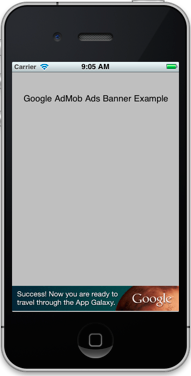
\includegraphics[scale=1]{Images/banner.png}
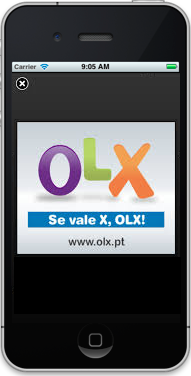
\includegraphics[scale=1]{Images/fullscreen.png}
Figure 1: Examples of advertisements

A banner advertisement is static and throughout the usage of an application takes up screen space that could otherwise host content of the application itself. In addition, banner advertisements are often flashing or making sound, further distracting the user from using the application.

Interstitial advertisements pop up from time to time throughout the usage of an application and temporarily stops the user from using the application altogether. Full-screen advertisements can be closed but it is often not intuitive how to do so without tapping on the advertisement itself and being redirected to the advertiser's website. In addition, opening and closing an interstitial advertisement often takes too long. it distracts the user and might get them out of the mood of using the application.

%: ----------------------- Mobile Cloud Middleware ------------------------

\section{Research Question}
%This section has three main parts: 
%1. a concise statement of the question that your thesis tackles 
%2. justification, by direct reference to section 3, that your question is previously unanswered
%3. discussion of why it is worthwhile to answer this question. 

The proposed solution for the problems that classical advertising methods have, is to display advertisements to the user in a way that the user could choose the location and size of the advertisement on the screen. This thesis tries to figure out whether this sort of mechanism is more user-friendly than mechanisms currently in use.

To do so such a mechanism is developed and implemented for a mobile application as a proof of concept. People are then asked to compare it to classical mobile advertising in terms of intrusiveness and their interest in the advertised product.

Advertisements are an inseparable part of mobile applications, but, as it stands, they are doing more harm than good...

%Summary of each chapter is MANDATORY
\section{Summary}
To counter the problems with the interoperability across multiple clouds, to perform data-intensive processing invocation from the handset and to introduce the platform independence feature for the mobile cloud applications, the following thesis discusses a Mobile Cloud Middleware (MCM). The middleware provides a unique interface for mobile connection and multiple internal interfaces and adapters, which manage the connection and communication between different clouds. The MCM capabilities for managing the resource intensive tasks can easily be envisioned in several scenarios which are discussed in further sections as case of study. 

% ---------------------------------------------------------------------------
%: -----------------------end of thesis sub-document---------------
% ---------------------------------------------------------------------------